%% Placeholder for chapter on linear equations and least squares
%%%zhipeng add the following part
%% Placeholder for chapter on linear equations and least squares




\section{Least Squares}
 
\begin{equation*}
Ax = y \,\,\,\,\,(*)
\end{equation*}
where $A\in \Re^{m\times n}$ is coefficient data matrix (known), $y\in \Re^m$ are constraints(known) and $x\in \Re^n$ are parameters (to choose).

There are three possibilities:

\begin{itemize}
	\item a) No $x\in \Re^n$ satisfies ($*$)
	
	\item b) Unique $x\in \Re^n$ satisfies ($*$)
	
	\item c) Many $x\in \Re^n$ satisfies ($*$)
\end{itemize}

(a) Existence:\\

Since $Ax\in \mathcal{R}(A)$, a solution will exist if $y\in \mathcal{R}(A)$

Test: 

1) $rank([A y]) = rank[A]$: solution to ($*$) exists

2) $rank([A y]) > rank[A]$: no solution to ($*$) exists\\

(b)/(c) If a solution exists, is it unique?

Assume a solution $\bar{x}$ exists s.t. $A\bar{x} = y$, any other solution $x$ myst also satisfy $Ax = y$. 

So 
\begin{align*}
Ax - A\bar{x} &= A(x -\bar{x}) = 0\\
x - \bar{x} &\in N(A)
\end{align*}

Any solution to ($*$) can be expressed as:
\begin{equation*}
x = \bar{x} + (x - \bar{x}) = \bar{x} + e
\end{equation*}
where $e\in N(A)$

So if there are solutions to ($*$), will be some affine sets:

\begin{equation*}
\mathcal{A} = \{x|x = \bar{x} + N(A), A\bar{x} = y \}
\end{equation*}
solution is unique if elements of $N(A)$ are all 0. $\bar{x}$ is any particular solution for $A\bar{x} =y$

The three cases typically bread down into a question about dimensions of $A\in \Re^{m\times n}$

\begin{itemize}
	\item 1) Overdetermined LS: more constraints than parameters $m>n$. Typically a solution does not exist. 
	
	\item 2) Square: Equal \# constraints \& parameters, typically $\exists$  a unique solution.
	
	\item 3) Underdetermined LS: Fewer constraints than parameters, $m<n$, typically many solutions
\end{itemize}

1) Overdetermined: $m > n$

Assume $A$ is full (column) rank, $rank(A) =n$. $A$ is tall, thin matrix. $dim(\mathcal{R}(A)) = n < m$. $y\in \Re^m$.\\

To find "closest" $Ax$ to $y$:

\begin{align*}
x^* &= arg \, min_{x\in \Re^n}||Ax - y||_2\\
min_{x\in \Re^{n}}||Ax - y|| &= min_{\hat{y}\in \mathcal{R}(A)}||\hat{y} - y||_2 =\prod_{\mathcal{R}(A)}(y)\\
\end{align*}

\begin{figure}
	\centering
	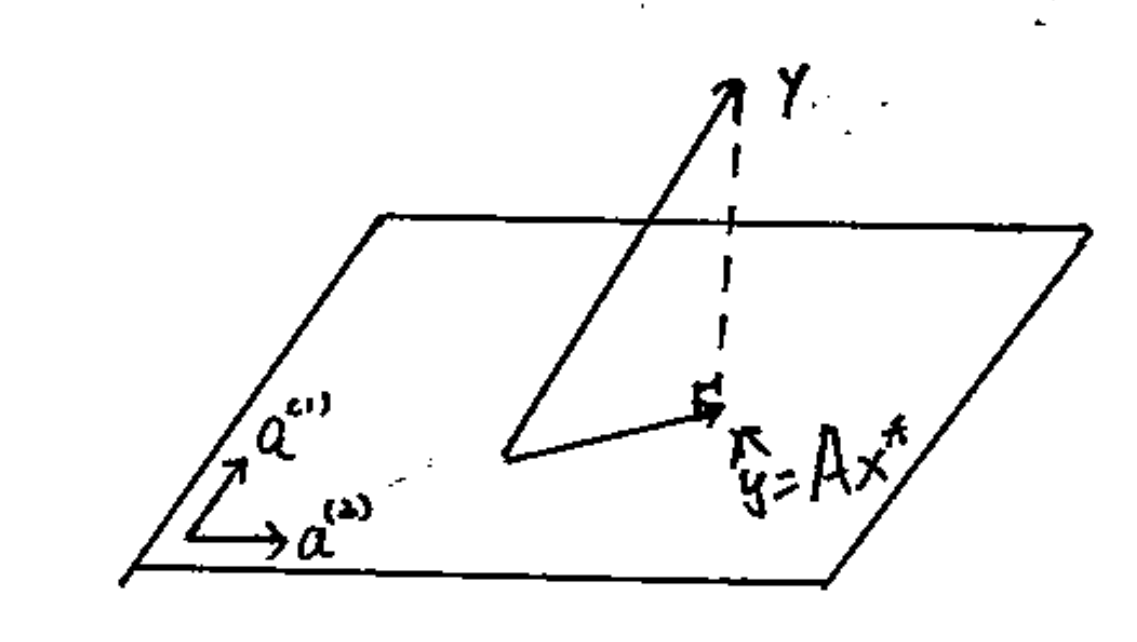
\includegraphics[width=2.1in,height=2.1in]{figures/ch06/figure1.png}
	%\caption{This is an inserted JPG graphic} 
	%\label{fig:graph} 
\end{figure}



From chapter2, 

\begin{equation*}
y^* = \sum^n_{i=1}x_i^*a^{(i)}
\end{equation*}
where 
$$ A =   
\left[
\begin{matrix}
a^{(i)} & ... & a^{(i)}
\end{matrix}
\right]
$$

Solve for $x^*$ via
\begin{equation*}
\sum^n_{i=1}x_1^*<a^{(k)}, a^{(i)}> = <a^{(k)}, y>, \forall k \in \{1,2,...,m \}
\end{equation*}

Stack up to get 

\begin{equation*}
A^TAx^* = A^Ty
\end{equation*}

There are 2 possibilities:

a) $A^TA$ is invertible.

b) $A^TA$ is not invertible.

a) 
\begin{align*}
x^* &= (A^TA)^{-1}A^Ty\\
\hat{y}^* &= A(A^TA)^{-1}A^Ty
\end{align*}

b) What happens if $A^TA$ is not invertible? 

\begin{align*}
\hat{y}^* &= A(A^TA)^{-1}A^Ty\\
&= A(V
\begin{bmatrix}
\Sigma & \textbf{0}
\end{bmatrix}
\mathcal{U}^T\mathcal{U}
\begin{bmatrix}
\Sigma \\
\textbf{0}
\end{bmatrix}
V^T)^{-1}A^Ty\\
&= A(V\Sigma^2V^T)^{-1}A^Ty\\
&= AV(\Sigma^{-1})^2V^TA^Ty\\
&= \mathcal{U}
\begin{bmatrix}
\Sigma \\
\textbf{0}
\end{bmatrix}
V^TV\Sigma^{-2}V^TV
\begin{bmatrix}
\Sigma & \textbf{0}
\end{bmatrix}
\mathcal{U}^Ty\\
&= \mathcal{U}
\begin{bmatrix}
\Sigma \\
\textbf{0}
\end{bmatrix}
\Sigma^{-1}\Sigma^{-1}
\begin{bmatrix}
\Sigma & \textbf{0}
\end{bmatrix}
\mathcal{U}^Ty
\end{align*}

Then we have:

\begin{align*}
y^{*} &= \mathcal{U}
\begin{bmatrix}
I_r\\
\textbf{0}
\end{bmatrix}
\begin{bmatrix}
I_r & \textbf{0}
\end{bmatrix}
\mathcal{U}^Ty\\
&= \mathcal{U}
\begin{bmatrix}
I_r& \textbf{0}\\
\textbf{0} & \textbf{0}
\end{bmatrix}
\mathcal{U}^Ty\\
&= \mathcal{U}
\begin{bmatrix}
I_r& \textbf{0}\\
\textbf{0} &  \textbf{0}
\end{bmatrix}
\begin{bmatrix}
<\mathcal{U}^{(1)}, y>\\
<\mathcal{U}^{(2)}, y>\\
...\\
<\mathcal{U}^{(m)}, y>
\end{bmatrix}\\
&= \sum^r_{i=1}<u^{(i)}, y>\mathcal{U}^{(i)}
\end{align*}

b) Uniquely determined:($m =n$)

\begin{equation*}
[A]x = y
\end{equation*}

\begin{equation*}
x^* = A^{-1}y
\end{equation*}

\begin{itemize}
	\item A full rank(columns\& rows)
	
	\item equal \# constraints \& parameters
	
	\item B/C A square \& full rank $A^{-1}$ exists
\end{itemize}

c) Underdetermined($m<n$)

\begin{itemize}
	\item A full row-rank
	
	\item rank(A) = m
	 
	\item A wide \& short matrix
	
	\item More parameters than constraints
	
	\item Hence many solutions
\end{itemize}

Idea: pick solution $x$ that satisfies($*$) and is shoetest

\begin{equation*}
x^* = arg \, min_{x\in \Re^n, Ax = y}||x||_2
\end{equation*}

\begin{equation*}
min_{Ax = y, x\in \Re^n}||x|| = min_{x\in \Re^n, x\in \mathcal{A}}||x - 0|| = \prod_{\mathcal{A}}(0)
\end{equation*}


\begin{figure}
	\centering
	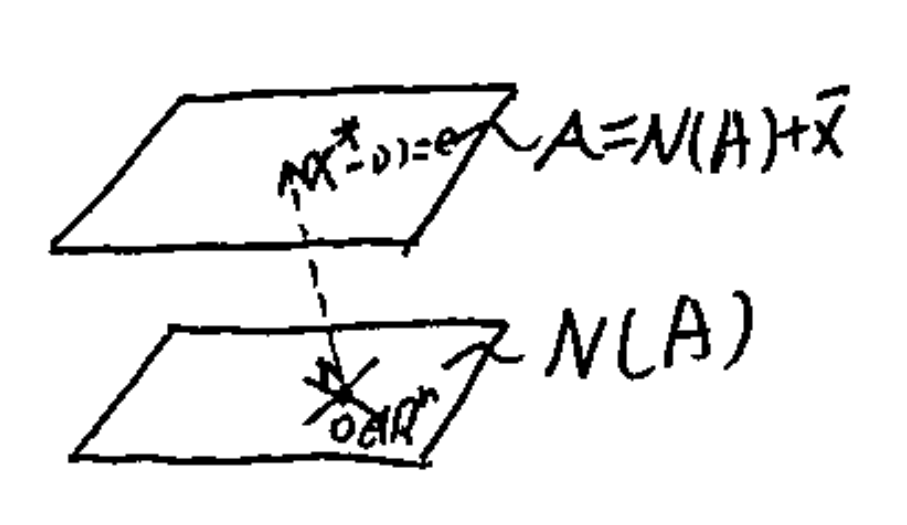
\includegraphics[width=2.1in,height=2.1in]{figures/ch06/figure3.png}
	%\caption{This is an inserted JPG graphic} 
	%\label{fig:graph} 
\end{figure}

To solve for $x^*$, note (from before) error vector 

\begin{align*}
e &= x^* - 0 = x^* \perp N(A)\\
x^* &\in N(A)^{\perp} = R(A^T)
\end{align*}

So we can write $x^* = A^T\alpha$ for some $\alpha \in \Re^m$. 
For $x^*$ to be in $\mathcal{A}$ it must be satisfies that $Ax^* = y$

Substituting in we get 

\begin{equation*}
y = Ax^* = AA^T\alpha
\end{equation*}

By assumption $A$ is full row rank so $AA^T$ is invertible.

\begin{align*}
\alpha^* &= (AA^T)y\\
x^T &= A^T(AA^T)y
\end{align*}

\begin{align*}
x^* &= A^T(AA^T)^{-1}y\\
&= A^T\left[\mathcal{U}
\begin{bmatrix}
\Sigma & \mathbf{0}
\end{bmatrix}
V^TV
\begin{bmatrix}
\Sigma\\
\mathbf{0}
\end{bmatrix}
\mathcal{U}^T\right]^{-1}y\\
&= A^T(\mathcal{U}\Sigma^2\mathcal{U}^T)^{-1}y\\
&= A^T\mathcal{U}\Sigma^{-2}\mathcal{U}^Ty\\
&= V
\begin{bmatrix}
\Sigma\\
\mathbf{0}
\end{bmatrix}
\mathcal{U}^T\mathcal{U}\Sigma^{-2}\mathcal{U}^Ty\\
&=V
\begin{bmatrix}
\Sigma^{-1} \\
\mathbf{0}
\end{bmatrix}
\mathcal{U}^Ty\\
&= V
\begin{bmatrix}
\Sigma^{-1}\\
\mathbf{0}
\end{bmatrix}
\begin{bmatrix}
<u^{(1)}, y>\\
...\\
<u^{(n)}, y>
\end{bmatrix}\\
&= \sum^r_{i=1}\frac{1}{\sigma_i}<u^{(i)}, y>V^{(i)}
\end{align*}





Below are written by Zhipeng for note on 26th Sep. \\


last time

solving linear system of equations Ax=y

1. over determined

$A^TAx=A^Ty$


2. under determined m<n

$X^* \in R(A^T)  $ 

3. invertiable





Today

interpretation and variations 


$min_x \Vert y-Ax\Vert_2$

1 approximate solution to y=Ax

$y^*=Ax^*$ best approx to solution in l2 space

closes point in R(A) to y

2. minimum perturbation of y to feasibility"

$y+\Delta y= y^*$

3. perturb both y and A to get feasibility

total least square

$\min_{\Delta y \Delta A} \Vert [\Delta A \Delta y] \Vert_F$, $\Delta A$ is m by n matrix and so $[\Delta A \Delta y]$ is m by n+1

% $\min_{\Delta y \Delta A} \Vert [\Delta A \Delta y] \Vert_F =  \lambda \Vert [\Delta A] \Vert_F + \Vert [\Delta y] \Vert_F $


$y+\Delta y\in R(A+\Delta A)$


4. Linear regression

$\Vert y-Ax\Vert ^2_2 = \sum_{i=1}^{m} ( y_i - <a^{(i)} , x>)^2$


examples

fit a line to $\{(0,6),(1,0),(2,0) \}={(a_i,y_i)}$

approximation of form $x_1+ax$

want $(y_i-x1+a_ix_i)^2 = r_i^2$

$x^*=(A^TA)^{-1}A^Ty=[5 , -3]^T$


$\hat{y}=x1^*+ax2^*=5-3a$            %so x1 and x2 are parameters


variants of ls

some residuals are more important than the others.

$\min \sum_{i=1}^{n} w_i r_i=\Vert W (y-Ax)\Vert ^2_2=\Vert Wy-WAx)\Vert ^2_2=\Vert \bar{y}-\bar{A} \Vert ^2_2$

can use a more general transform 

$\Vert W (y-Ax)\Vert ^2_2 = (y-Ax)^TW^TW(y-Ax)=r^TW^TWr$

$x^*=(A^TW^TWA)^{-1}A^TWW^Ty$




weighted least square (ls) 

when W is diagonal 

figure here

when W is PSD (rotation)

figure here




Regularization LS

l2 regularized LS

in ls $x*=\arg_x\in\reals_{n} \min \Vert Y-Ax\Vert ^2_2$

and no preference for any specific x over any other, and often x is a vector of resources consumed.

regularized ls

$x*=\arg_x\in\reals_{n} \min \Vert Y-Ax\Vert ^2_2 + \gamma \Vert x\Vert ^2_2$, where $\gamma$ is a non negative scalar


To solve regularized ls

$u\in\reals_{n}, v\in\reals_{m}$


Define

%\bar{A}=

$\Vert Y-Ax\Vert ^2_2 + \gamma \Vert x\Vert ^2_2=\Vert \bar{A}x-\bar{y}\Vert^2_2$

$x^*=(\bar{A}^TA)^{-1}\bar{A}^T\bar{y}=(A^TA+\gamma I)^{-1}A^Ty$


tiknon regularization

content here


Visualize regularized LS

$\min \Vert Ax-y\Vert_2^2 +\gamma\Vert x\Vert^2_2$

recall $x^*=[5 -3]^T$, and $\Vert Ax^*-y\Vert = 6$

figure here


Draw level set for some picture

figure here

figure here



$c_1=\Vert Ax-y\Vert^2_2=\Vert A(x-x_s^*+x_s^*)-y\Vert^2_2=\Vert (Ax_s^*-y)-A(x-x_s^*)\Vert^2_2=\Vert (Ax_s^*-y)\Vert^2_2 - \Vert A(x-x_s^*)\Vert^2_2$

The first term on r.h.s is a scalar 6, so we focus on the second term now.

$\Vert A(x-x_s^*)\Vert^2_2= (x-x_s^*)^T A^TA (x-x_s^*)$ 

Note that $A^TA$ is a PSD matrix.


Understand geometry level set of $\Vert A(x-x_s)\Vert^2_2$ via eigenvector of PSD matrix $A^TA$


$A^TA=$

figure here

















Above are written by Zhipeng for note on 26th Sep. \\

Below are written by Yanxiao starts on 9th Oct. \\

\subsection{Least Squares}
\begin{equation*}
x^* = arg\, min_{x\in \Re^n}||y-Ax||_2^2 \,\,\,\,\, (*)
\end{equation*}

\begin{itemize}
	\item Standard LS variant in ($*$) weights all elements of error vector equally.(weighted LS)
	
	\item Standard LS measures error along standard coordinate system.(change coordinate system)
	
	\item Standard LS ignores that certain elements of $x$ may "cost" more than others.(regularization)
\end{itemize}

\subsection{"Tikhanov regularization"}
\begin{equation*}
x^* =arg\,min_{x\in \Re^n}||w_1(y-Ax)||_2^2 + ||w_2(x - x^{(0)})||_2^2
\end{equation*}\\

We do a simple example:

\begin{equation*}
x^* = arg\,min_{x\in \Re^n}||y-Ax||_2^2 + \gamma||x||_2^2
\end{equation*}

\begin{figure}
	\centering
	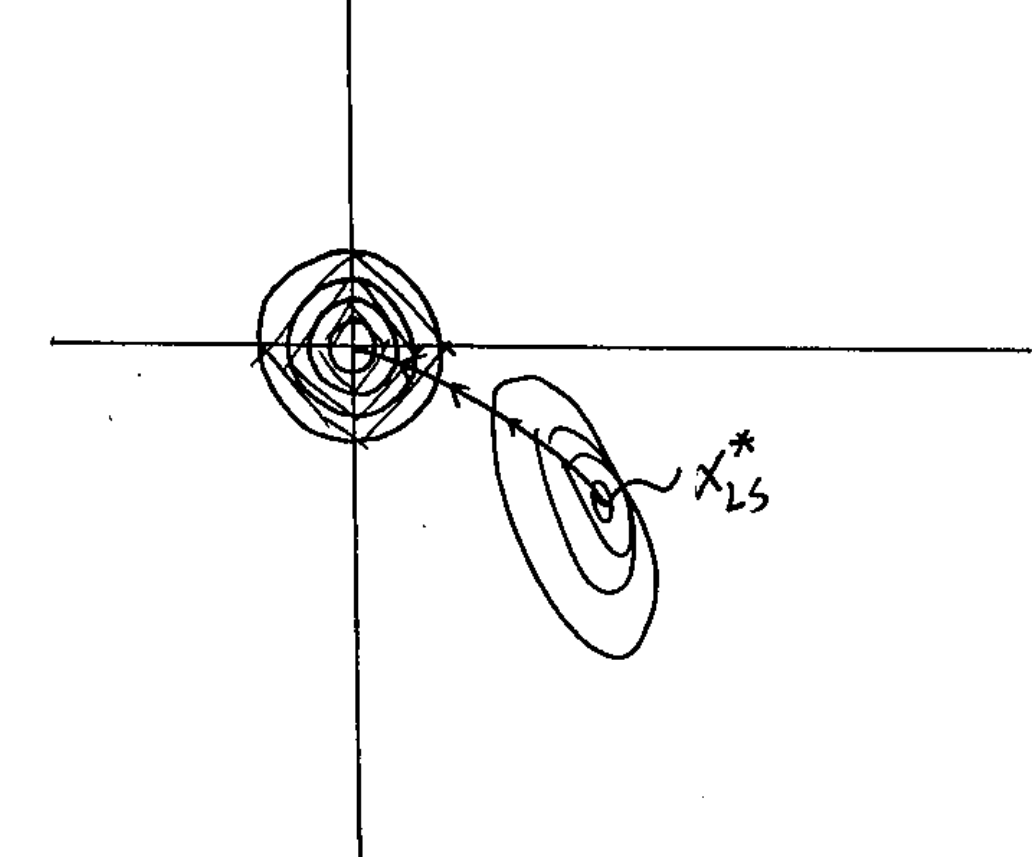
\includegraphics[width=2.1in,height=2.1in]{figures/ch06/figure4.png}
	%\caption{This is an inserted JPG graphic} 
	%\label{fig:graph} 
\end{figure}

Look at form of optional solution to 

\begin{align*}
x^* &= arg\,min_{x\in \Re^n}||y-Ax||_2^2 + \gamma||x||^2_2\\
&= (A^TA + \gamma I)^{-1}A^Ty\\
\hat{y}&= Ax^* = A(A^TA + \gamma I)^{-1}A^Ty\\
\end{align*}
apply SVD of A
\begin{equation*}
A = \mathcal{U}\tilde{\Sigma}V^T
\end{equation*}

First thing is to analyze $(A^TA + \gamma I)^{-1}$:

\begin{align*}
(A^TA + \gamma I)^{-1} &= (V\tilde{\Sigma}^T\mathcal{U}^T\mathcal{U}\tilde{\Sigma}V^T + \gamma I)^{-1}\\
&= (V
\begin{bmatrix}
\Sigma^T & 0\\
0 & 0\\
\end{bmatrix}
\begin{bmatrix}
\Sigma & 0\\
0 & 0\\
\end{bmatrix}
V^T + \gamma I)^{-1}\\
&=(V
\begin{bmatrix}
\Sigma^2 & 0\\
0  & 0
\end{bmatrix}
V^T + \gamma VV^T
)^{-1}\\
&= (V(
\begin{bmatrix}
\Sigma^2 & 0\\
0 & 0
\end{bmatrix}
+\gamma I)V^T)^{-1}\\
&= V
\left[
\begin{array}{c|c}
\Sigma^2+\gamma I_r&  \\ \hline 
& I_{n-r}
\end{array}
\right]
V^T\\
&=
V
\left[
\begin{array}{c|c}
(\Sigma^2+\gamma I_r)^{-1}&  \\ \hline 
& (I_{n-r})^{-1}
\end{array}
\right]
V^T\\
&=
V
\left[
\begin{array}{c|c}
\begin{matrix}
\frac{1}{\sigma_1^2+\gamma} & &\\
&\ddots&\\
&&\frac{1}{\sigma_r^2+\gamma}
\end{matrix}&  \\ \hline 
& \begin{matrix}
\frac{1}{\gamma} & &\\
&\ddots&\\
&&\frac{1}{\gamma}
\end{matrix}
\end{array}
\right]
V^T
\end{align*}

%\begin{matrix}
%	\frac{1}{\sigma_1^2+\gamma} & &\\
%	&...&\\
%	&&\frac{1}{\sigma_r^2+\gamma}
%\end{matrix}


%\left[
%\begin{array}{c|c}
%	\begin{matrix}
%		\frac{1}{\sigma_1^2+\gamma} & &\\
%		&...&\\
%		&&\frac{1}{\sigma_r^2+\gamma}
%	\end{matrix}&  \\ \hline 
%	& \begin{matrix}
%		\frac{1}{\gamma} & &\\
%		&...&\\
%		&&\frac{1}{\gamma}
%	\end{matrix}
%\end{array}
%\right]



\begin{align*}
y^* &= Ax^* = A(A^TA + \gamma I)^{-1}A^Ty\\
&= \mathcal{U}\tilde{\Sigma}V^T\left(V
\left[
\begin{array}{c|c}
\begin{matrix}
\frac{1}{\sigma_1^2+\gamma} & &\\
&\ddots&\\
&&\frac{1}{\sigma_r^2+\gamma}
\end{matrix}&  \\ \hline 
& \begin{matrix}
\frac{1}{\gamma} & &\\
&\ddots&\\
&&\frac{1}{\gamma}
\end{matrix}
\end{array}
\right]
V^T\right)V\tilde{\Sigma}\mathcal{U}^Ty\\
&= \mathcal{U}
\begin{bmatrix}
\Sigma & 0\\
0 & 0
\end{bmatrix}
\left[
\begin{array}{c|c}
\begin{matrix}
\frac{1}{\sigma_1^2+\gamma} & &\\
&\ddots&\\
&&\frac{1}{\sigma_r^2+\gamma}
\end{matrix}&  \\ \hline 
& \begin{matrix}
\frac{1}{\gamma} & &\\
&\ddots&\\
&&\frac{1}{\gamma}
\end{matrix}
\end{array}
\right]
\begin{bmatrix}
\Sigma^T & 0\\
0 & 0
\end{bmatrix}
\mathcal{U}^Ty\\
&= \mathcal{U}
\left[
\begin{array}{c|c}
\begin{matrix}
\frac{sigma_1^2}{\sigma_1^2+\gamma} & &\\
&\ddots&\\
&&\frac{sigma_r^2}{\sigma_r^2+\gamma}
\end{matrix}&  \\ \hline 
& 0
\end{array}
\right]
\mathcal{U}^Ty
\\
&= \mathcal{U}
\left[
\begin{array}{c|c}
\begin{matrix}
\frac{sigma_1^2}{\sigma_1^2+\gamma} & &\\
&\ddots&\\
&&\frac{sigma_r^2}{\sigma_r^2+\gamma}
\end{matrix}&  \\ \hline 
& 0
\end{array}
\right]
\begin{bmatrix}
<u^{(1)}, y>\\
<u^{(2)}, y>\\
\vdots\\
<u^{(m)}, y>
\end{bmatrix}\\
&=\mathcal{U}
\begin{bmatrix}
\frac{\sigma_1^2}{\sigma_1^2+\gamma}<u^{(1)}, y>\\
\vdots\\
\frac{\sigma_r^2}{\sigma_r^2+\gamma}<u^{(r)}, y>\\
0\\
\vdots\\
0
\end{bmatrix}\\
&= \sum^r_{i=1}\frac{\sigma_i^2}{\sigma_i^2 + \gamma}<u^{(i)}, y>u^{(i)}
\end{align*}\\

By considering

\begin{equation*}
\sum^r_{i=1}\frac{\sigma_i^2}{\sigma_i^2 + \gamma}<u^{(i)}, y>u^{(i)}
\end{equation*}

We should note:

\begin{itemize}
	\item $\frac{\sigma_i^2}{\sigma_i^2 + \gamma}$: scaling is changed by regularization. If $\gamma = 0$, then  $\frac{\sigma_i^2}{\sigma_i^2 + \gamma} = 1$ and get back standard LS. If $\gamma > 0$, it's shrinkage. 
	
	\item $<u^{(i)}, y>$: projection of data vector $y$ along that $i^{th}$ direction. 
	
	\item $u^{(i)}$: component of approximation along $i^{th}$ direction or $i^{th}$ basis element. 
\end{itemize}



